\documentclass[a4paper]{scrreprt}

\usepackage[german]{babel}
\usepackage[utf8]{inputenc}
\usepackage[T1]{fontenc}
\usepackage{ae}
\usepackage[bookmarks,bookmarksnumbered]{hyperref}
\usepackage{graphicx}
\usepackage{float}
\usepackage{color}
\usepackage{pdfpages}
\graphicspath{ {Images/} }
\setcounter{secnumdepth}{5}

\begin{document}

    \begin{flushright}
        
\includegraphics[scale = 0.7]{kit-logo.jpg}\\[0.5cm]
        % 
\includegraphics[scale = 1]{teco.jpg}
    \end{flushright}
    % 
\includegraphics[scale = 0.5]{kit-logo.jpg} \hspace{4cm} 
\includegraphics[scale = 1]{teco.jpg}
    \vspace*{2cm}

    \begin{center} \large

        Praxis der Softwareentwicklung
        \vspace * {1.5cm}

        \textbf{\huge Mind Rate}

        \vspace*{1cm}


        {\Large Ein interaktives System mit Android-Client f\"ur Studien nach Experience-Sampling-Method (ESM)}

        \vspace*{1cm}

        \textbf{\Large Implementierung}
        \vspace*{2cm}

        Shanshan Du, Yi Ge, Renhan Lou, Ruoheng Ma, Haobin Tan
        \vspace*{1cm}

        19. Februar 2017
        \vspace*{2.5cm}

        Betreuung: Anja Exler, Dr. Andrea Schankin\\[0.5cm]
        Forschungsgruppe TECO: Technology for Pervasive Computing\\[0.5cm]

        Karlsruher Institut für Technologie
    \end{center}
    \thispagestyle{empty}

    \tableofcontents

    \chapter{Einleitung}

        Nach der Entwurfsphase haben wir vollständige klassendiagramme der Server-Seite und Android-App erhalten. Wir haben die Struktur der ganzen Software auch festgelegt. In der Implementierungsphase wird die Software auch in zwei Teile eingeteilt. Der erste Teil ist eine Android Applikation, die von der Probanden benutzt werden können. Der zweite Teil ist ein Web-Interface, das von Studienleiter benutzt werden können. Zusätzlich liegt eine Datenbank auf dem Server vor, um die Daten zwischen zwei Seite zu übertragen.





    \newpage
    \chapter{Änderungen am Entwurf}


        \section{Android Applikation}

            Die neu hinzufügte Pakete und Klassen werden mit \textcolor{green}{grün} markiert.

            \subsection{Überblick}

                \begin{figure}[H]
                    \centering
                    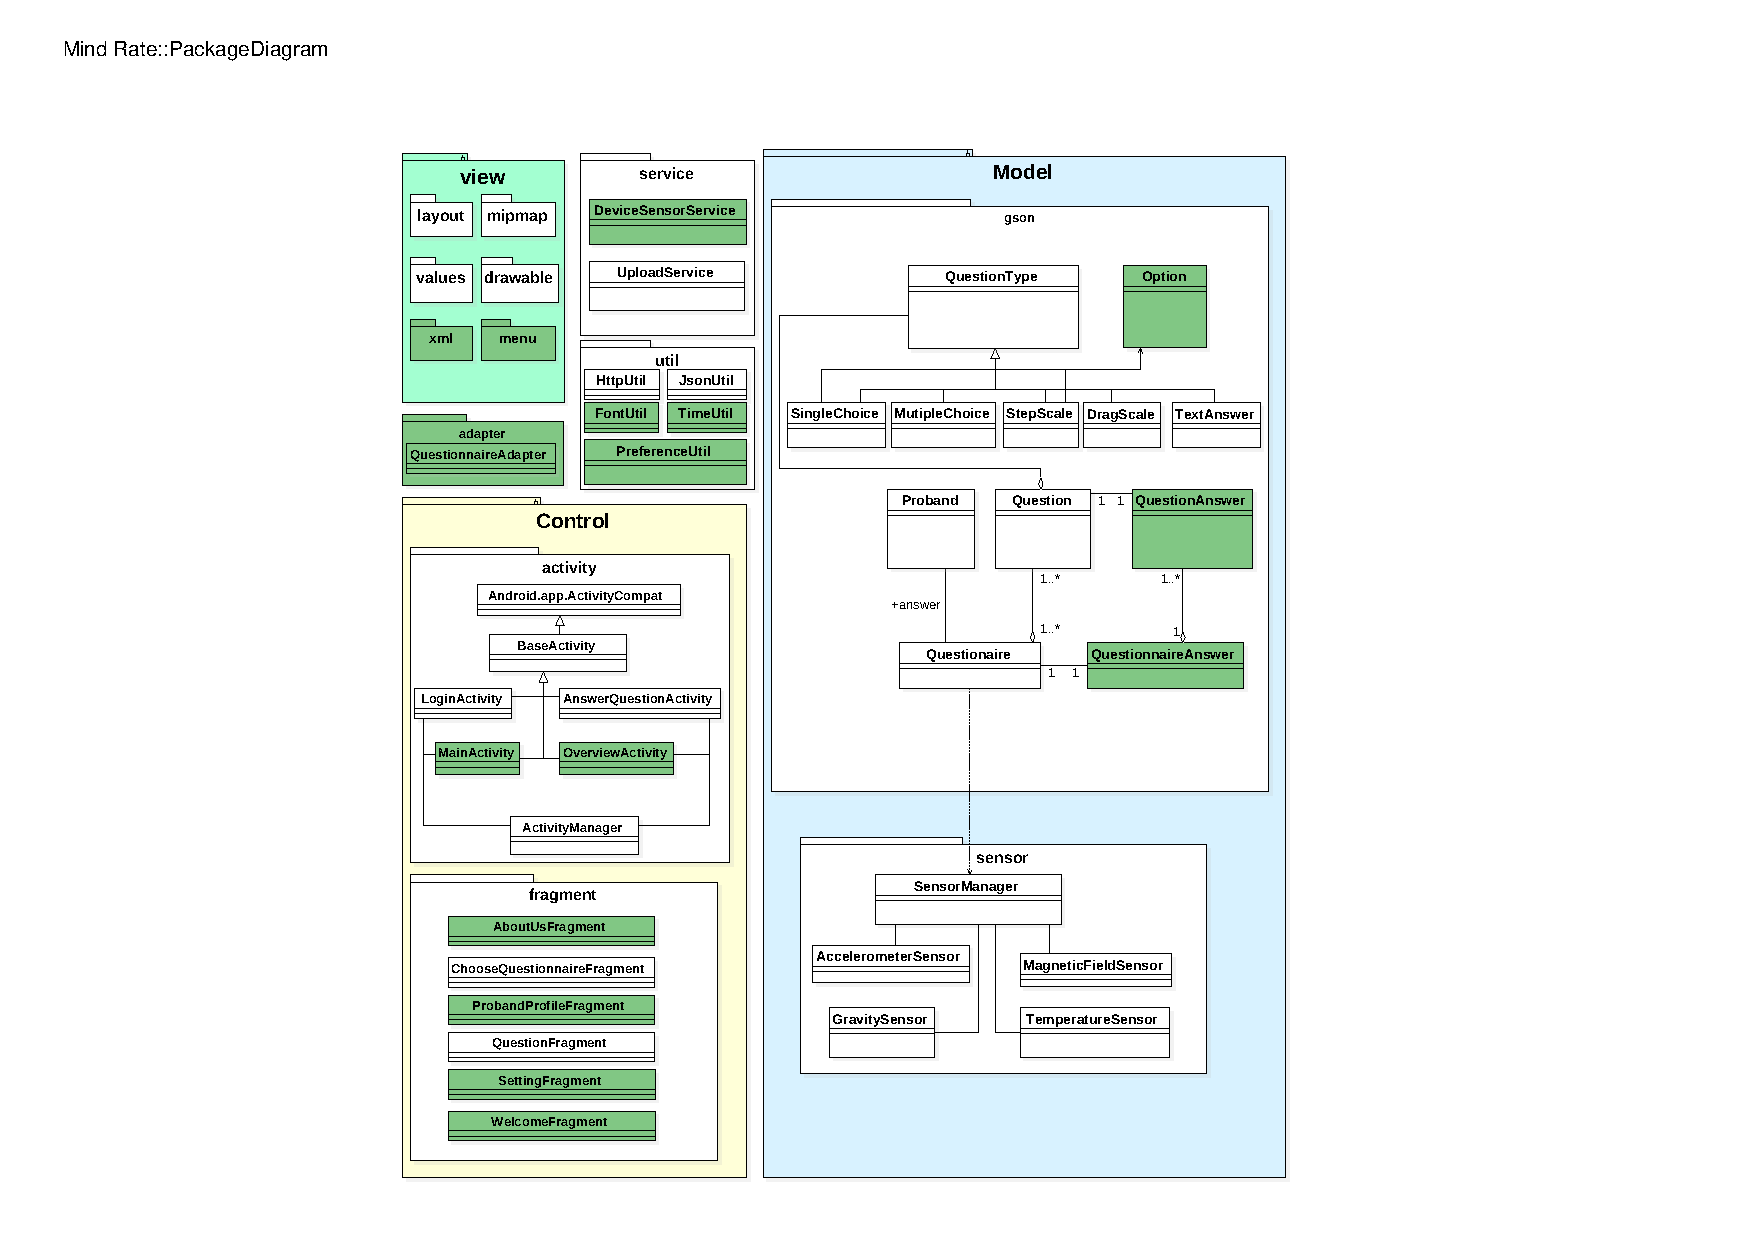
\includegraphics[scale = 1.0]{PackageDiagram.pdf}
                    \caption{Überblick}
                \end{figure}



            \subsection{package activity}


            \subsection{package fragment}
            \subsection{package gson}
                \begin{figure}[H]
                    \centering
                    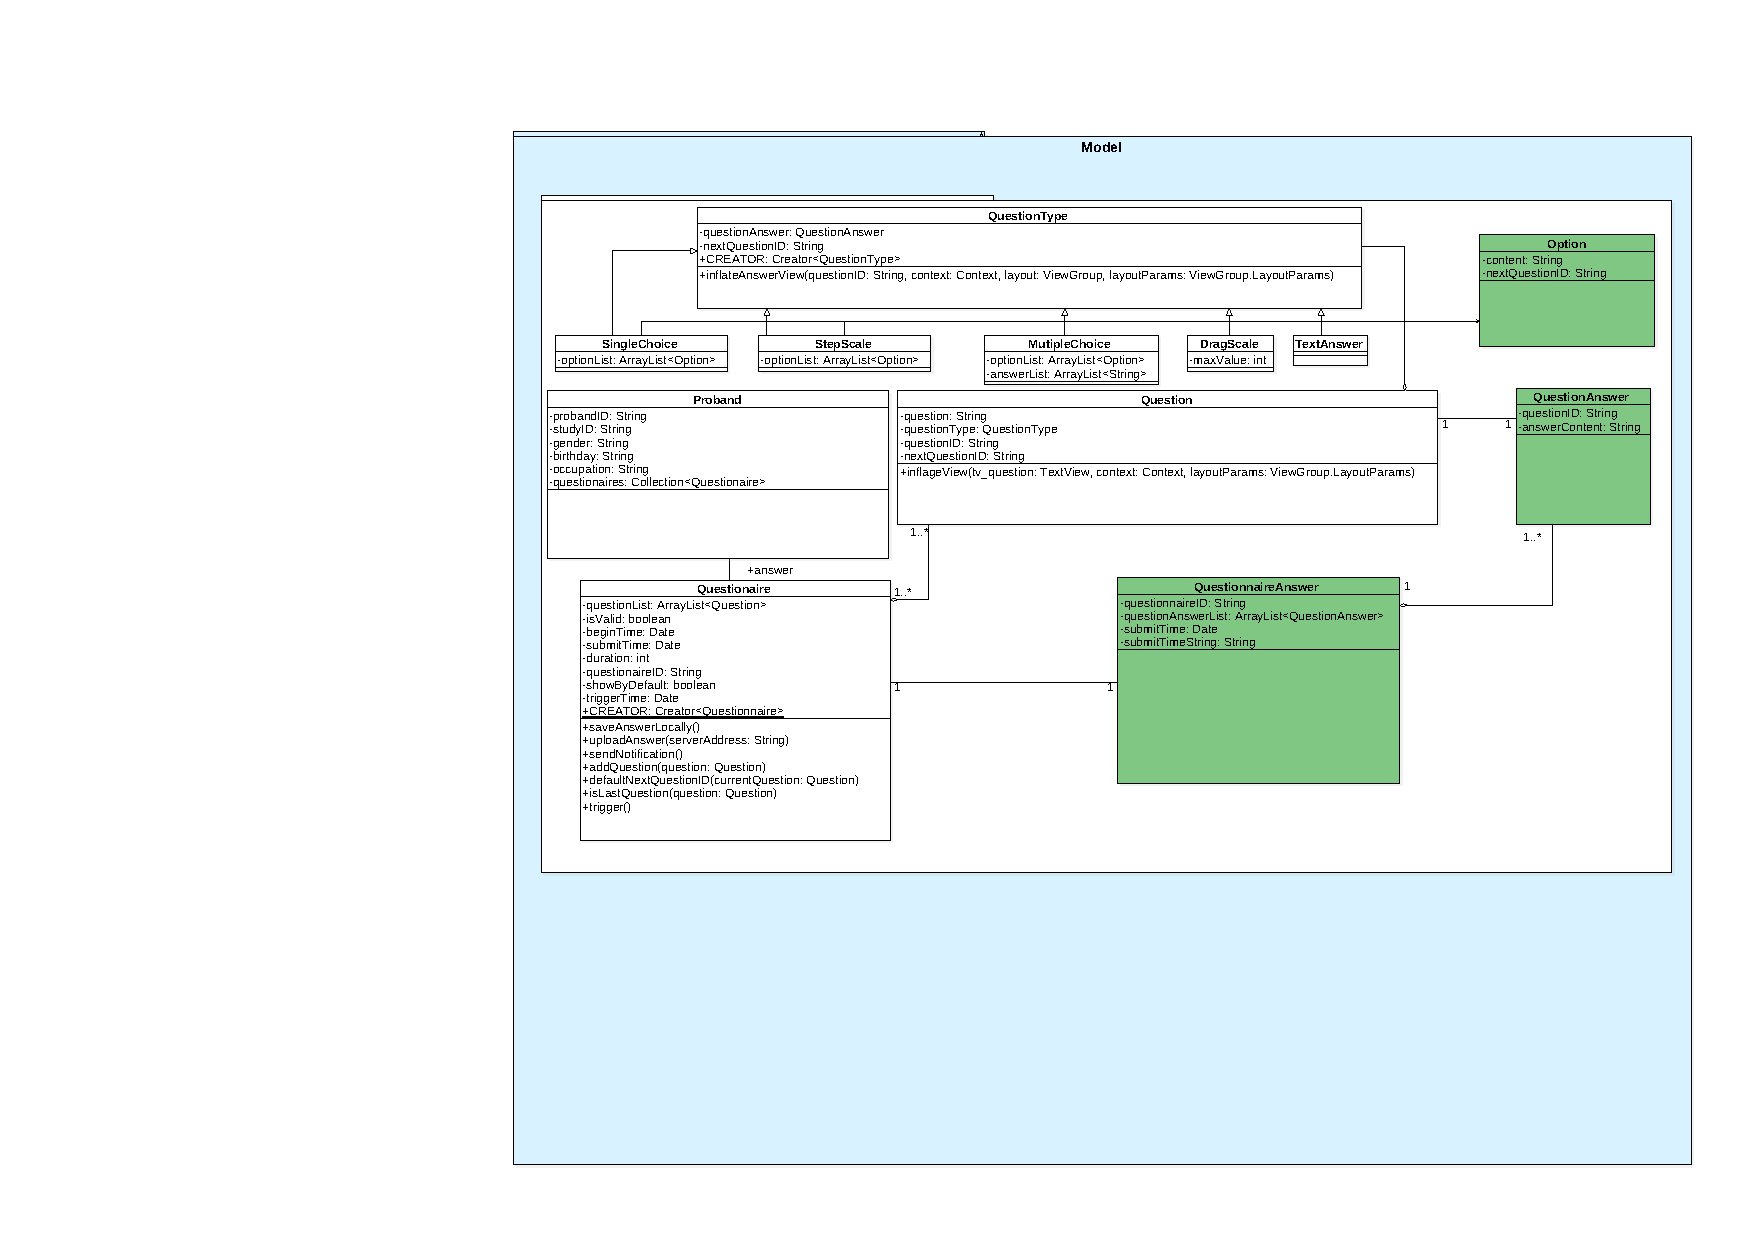
\includegraphics[scale = 0.8]{gson.pdf}
                    \caption{Package gson}
                \end{figure}
            \subsection{package service}
            \subsection{package util}


        \section{Server}
            \begin{itemize}
                \item Ersetzen von \texttt{StudyDirector}-Klasse durch \texttt{django.contrib.auth.models.User}-Klasse

                \item Die Zugehörigkeit zwischen Studienleiter und Studien werden durch \texttt{owner}-Attribut der \texttt{Study}-Klasse und Objekt-Niveau-Erlaubnis von Django realisiert

                \item Ersetzen aller Datentypen der Objekt-Attributen durch entsprechende Unterklassen der \texttt{django.db.models.Field}-Klasse, um Daten in die Datenbank zu speichern

                \item \texttt{ChoiceQuestion}-Klasse wird zu \texttt{SingleChoiceQuestion}- und \texttt{MultiChoiceQuestion}-Klassen geteilt

                \item Hinzufügen von \texttt{ChoiceOption}-Klasse, um Optionen der Ein- und Mehrfachauswahlen zu modellieren

                \item Das \texttt{FollowUpQuestion}-Attribut liegt nicht mehr in \texttt{ChoiceQuestion}-Klasse, sondern in \texttt{ChoiceOption}-Klasse, um verschiedene Folgefragen per Option zu ermöglichen

                \item Hinzufügen von \texttt{ProbandInfoQuestionnaire}-Klasse: der Studienleiter kann selbst entscheiden, welche demographische Informationen aus den Probanden zu sammeln

                \item Informationen der Probanden werden in mehrere \texttt{ProbandInfoCell}-Objekte gespeichert, und danach durch \texttt{ForeignKey} zu einem \texttt{Proband}-Objekt gelinkt werden

                \item Ersetzen von \texttt{linearAcceleration}-, \texttt{gravity}-, \texttt{rotation}- und \texttt{orientation}-Attributen der \texttt{TriggerEvent}-Klasse durch das Android-User-Activity-API-basierte \texttt{user\_activity}-Attribut

                \item Die \texttt{light}-, \texttt{relative\_humidity}-, \texttt{proximity} und \texttt{air\_pressure}-Sensoroptionen nehmen keine exakte Zahl mehr, sondern einen 5-stufigen Wert zwischen “very high” und “very low”


            \end{itemize}
            
            \subsection{Klassendiagramm}
                \begin{figure}[H]
                    \centering
                    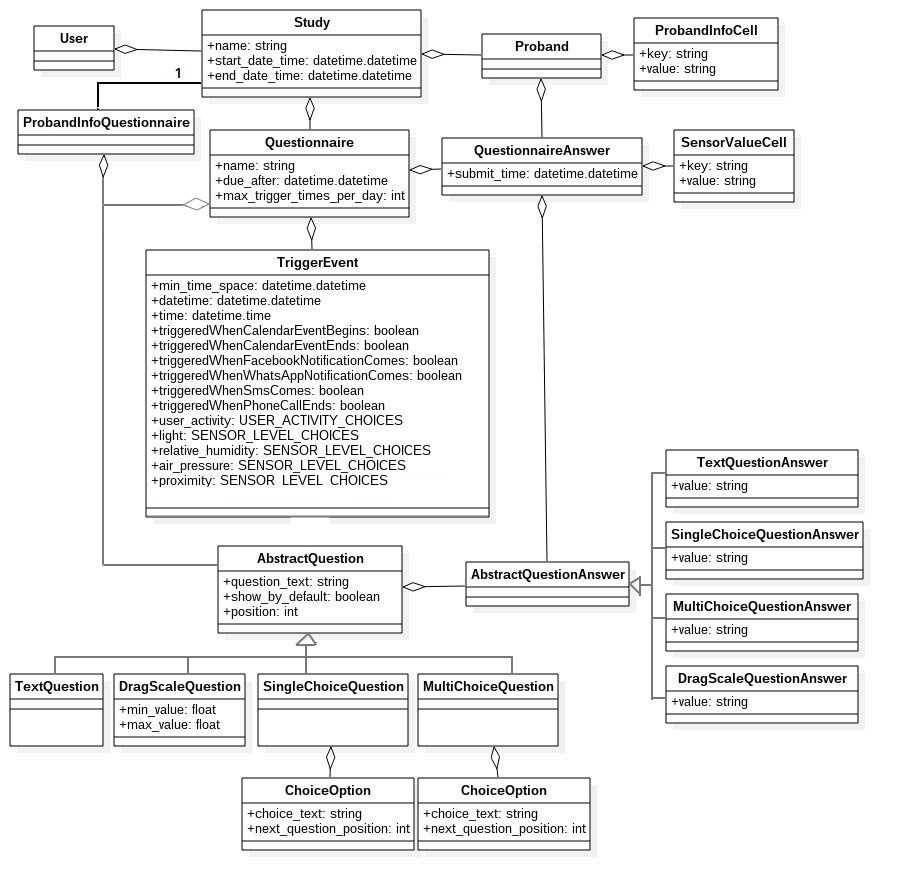
\includegraphics[scale = 0.5]{class_diagram_server.jpg}
                    \caption{Class diagram server side}
                \end{figure}


        \newpage
    \chapter{Implementierte Muss- und Wunschkriterien}


        \section{Android Applikation}





        \section{Server}


           \newpage
    \chapter{GANTT Diagramm}

        \section{Android Applikation}
        \begin{figure}[H]
                \centering
                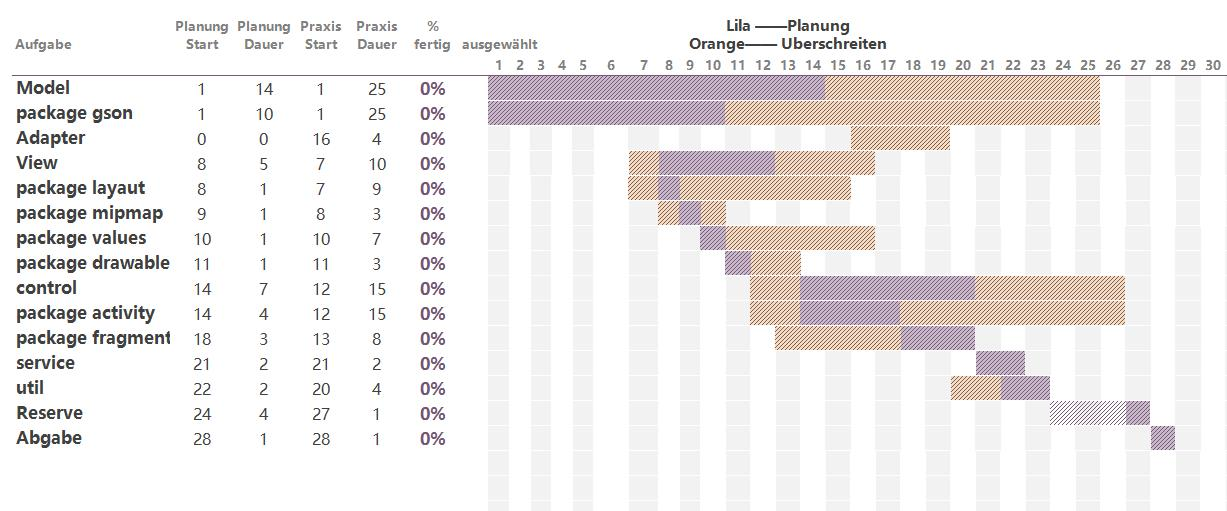
\includegraphics[scale = 0.65]{aktuelleAndroidAppZeitplanung.jpg}
                \caption{Aktueller Zeitaufwand der Android App }
        \end{figure}
        \begin{itemize}   
         \item Verzögerung
                 \begin{itemize}
                    \item Model
                    \begin{itemize}
                        \item Neue Klassen werden dem Paket gson hinzugefügt. Z.B. TriggerEventManagerment und AllSensorEventListener. Viele Funktionen und Methoden werden geändert und erzeugt.
                     \end{itemize}
                  \end{itemize}  
                  \begin{itemize}
                        \item Adapter
                            \begin{itemize}
                            \item Ein neues Paket Adapter wird erzeugt.
                            \end{itemize}
                  \end{itemize} 
                  \begin{itemize}
                        \item View
                            \begin{itemize}
                            \item Paket layout und Paket values sind zeitaufwendig.
                            \end{itemize}
                  \end{itemize}
                   \begin{itemize}
                        \item control
                            \begin{itemize}
                            \item Neue Klassen werden dem Paket activity hinzugefügt, und der Teil der Sensoren wird darin implementiert.
                            \end{itemize}
                  \end{itemize} 
                  \begin{itemize}
                        \item service
                            \begin{itemize}
                            \item  Diese Aufgabe ist rechtzeitig fertig.
                            \end{itemize}
                  \end{itemize} 
                  \begin{itemize}
                        \item util
                            \begin{itemize}
                            \item Neue Klassen werden dem Paket util hinzugefügt.
                            \end{itemize}
                  \end{itemize}                                                
            
        \end{itemize}
       

        \section{Server}

       \newpage

    \chapter{Übersicht zu unit tests}

        \section{Android Applikation}

        \section{Server}

    \newpage

\end{document}
